\chapter{Desarrollo de la Solución}
\label{sec:desarrollo}

\section[Proceso de Desarrollo]{Proceso de Desarrollo}

\subsection{Versionado de código}

\subsection{Integración Continua}

\subsection{Tests}

\section[Núcleo]{Núcleo}

El núcleo se encarga de administrar los datos no sensibles de los alumnos y sus materias cursadas, las inscripciones, planes de estudio con sus créditos, recorrido obligatorio y recomendado de inscripciones, entre otros.
El núcleo tiene la capacidad de servir dichos datos para que sean consumidos por los usuarios que tengan los permisos correspondientes.
Los usuarios tienen permisos asignados que corresponden con la carrera a la que pertenecen, que les permiten consultar datos de dicha carrera. 






\begin{figure}[h!]
  \centering
    
\includegraphics[scale=0.5]{images/nucleo/nucleo-fondoblanco.png}
  \captionof{figure}{Logo del Núcleo}
  \label{fig:django}
\end{figure}

\subsection{Tecnologías}

El Núcleo fue desarrollado con Python 3.6, usando el framework web Django en su versión 3.0.
Django incluye un administrador (django-admin) que genera automáticamente los listados, la creación, la edición y el borrado de los modelos desarrollados. Además, trae un sistema de autenticación de usuarios que facilita la tarea de autorizar usuarios a través de permisos.
Se eligió django-rest-framework para crear una API REST para que otros servicios puedan consultar o crear datos.
Usando django-rest-framework-simplejwt, se implementó JWT. Es decir, todo servicio que quiera acceder a los datos tendrá que pedir un token. Si éste está habilitado para consumir datos, se le proveerá de dicho token.

\subsection{Administración de los datos}

Los usuarios que tengan permiso para ingresar al Administrador, pueden hacerlo mediante una pantalla de Login como muestra la figura ~\ref{fig:nucleo-login}.
Una vez ingresados, pueden ver la pantalla principal del administrador, como muestra la figura ~\ref{fig:nucleo-home}, donde tienen diferentes menús para utilizar los datos. Tienen acceso a diferentes listados (figura ~\ref{fig:nucleo-listado}), creación, edición y borrado (figura ~\ref{fig:nucleo-edicion}).
Los usuarios tienen también la posibilidad de importar planillas de datos (figura ~\ref{fig:nucleo-importador}).

\subsubsection{Usuarios y permisos}

Para resolver la autenticación y autorización en el administrador de contenidos, se usó el sistema de autenticación que viene embebido en Django.
Este sistema provee una manera de asignar permisos a usuarios específicos o grupos de usuarios. Estos permisos se dividen en:
\begin{outline}
    \1 El acceso a ver objetos está limitado a los usuarios que tengan los permisos \textit{view} o \textit{change}.
    \1 El acceso a ver los formularios para agregar elementos, está limitado a los usuarios que tengan el permiso \textit{add} para ese tipo de objetos.
    \1 El acceso a ver los listados, ver los formularios de edición y la posibilidad de editar, están limitados a los usuarios que tengan el permiso \textit{change} para ese objeto en particular.
    \1 El acceso a eliminar un objeto está limitado a los usuarios que tengan el permiso \textit{delete}.
\end{outline}

\subsubsection{Grupos de usuarios}

Django provee una forma de categorizar usuarios a los que se les puede aplicar permisos llamado \textit{grupo}. Un usuario puede pertenecer a muchos grupos.
Un usuario que pertenezca a un grupo, automáticamente tiene los permisos asignados a dicho grupo.
Otra particularidad de esto, además de los permisos, es que pueden servir para extender las funcionalidades. Por ejemplo, si quisiera que un grupo fuese "Usuarios de LIDS", podría asignarle a ese grupo la carrera "LIDS" para que sólo pudieran ver datos relacionados a su carrera y no a otras.


\subsection{Importadores}

En el caso que los usuarios tengan la necesidad de importar los datos a través de planillas, se realizaron diferentes importadores para esta tarea (~\ref{fig:nucleo-importador}).
Estos importadores son:
\begin{outline}
\2 Carreras
\2 Planes de estudio con sus materias
\2 Prerrequisitos obligatorios y recomendados de materias
\2 Alumnos con sus datos personales
\2 Materias cursadas por alumnos
\2 Inscripciones a materias
\end{outline}

\subsection{API}

Se diseñó una API para consultar datos a través de distintas URIs (tabla ~\ref{tab:tabla_api}), para las cuales se necesita de un token (tabla ~\ref{tab:tabla_token}).
Dicho token es de la forma:

\textit{eyJ0eXAiOiJKV1QiLCJhbGciOiJIUzI1NiJ9.} \break 
\textit{eyJ0b2tlbl90eXBlIjoiYWNjZXNzIiwiZXhwIjoxNTg5Mjk2NjAyLCJ}\break 
\textit{qdGkiOiJhMTAzMmI2YzdiN2Y0ZjlkODc5NzI0NGViZTQxYTk5YSIsInV}\break 
\textit{zZXJfaWQiOjEsImNhcnJlcmFzIjpbIlciXSwiY2FycmVyYXNfbGFiZWwi} \break \textit{OltbIlciLCJMaWNlbmNpYXR1cmEgZW4gRGVzYXJyb2xsbyBkZSBTb2Z0d2}\break 
\textit{FyZSJdXSwidXNlcm5hbWUiOiJhZG1pbiJ9}.\break 
\textit{xWWi-sDFQ6I-CK0xC7tmkTw1mXRmMhFFse6\_qnKBiaE}

\break
El \textit{Header} del token tiene la siguiente información:
\begin{lstlisting}[language=json,firstnumber=1]
{
"typ": "JWT",
"alg": "HS256"
}
\end{lstlisting}
\break
Para el caso del \textit{Payload}, se tiene la siguiente información indicando precisamente qué carreras puede consultar el usuario:
\begin{lstlisting}[language=json,firstnumber=1]
{
  "token_type": "access",
  "exp": 1589296602,
  "jti": "a1032b6c7b7f4f9d8797244ebe41a99a",
  "user_id": 1,
  "carreras": [
    "W"
  ],
  "username": "admin"
}
\end{lstlisting}

\subsubsection{Ejemplo de pedido}
Si quisiera saber qué materias hay dentro de una carrera en un plan determinado, deberia hacer de la siguiente manera:

\begin{lstlisting}[language=bash]
GET 'https://url.del.nucleo/api/carreras/W/planes/2015/'
--header Authorization: Bearer <token>
\end{lstlisting}

El resultado tendrá la siguiente forma:

\begin{lstlisting}[language=json,firstnumber=1]
[{
        "id": 54,
        "materia": "Taller de Trabajo Intelectual",
        "plan": 2015,
        "nucleo": "",
        "creditos": 4,
        "area": "Taller",
        "codigo": "00751"
    },
    ...
]
\end{lstlisting}

\begin{figure}[h!]
  \centering
    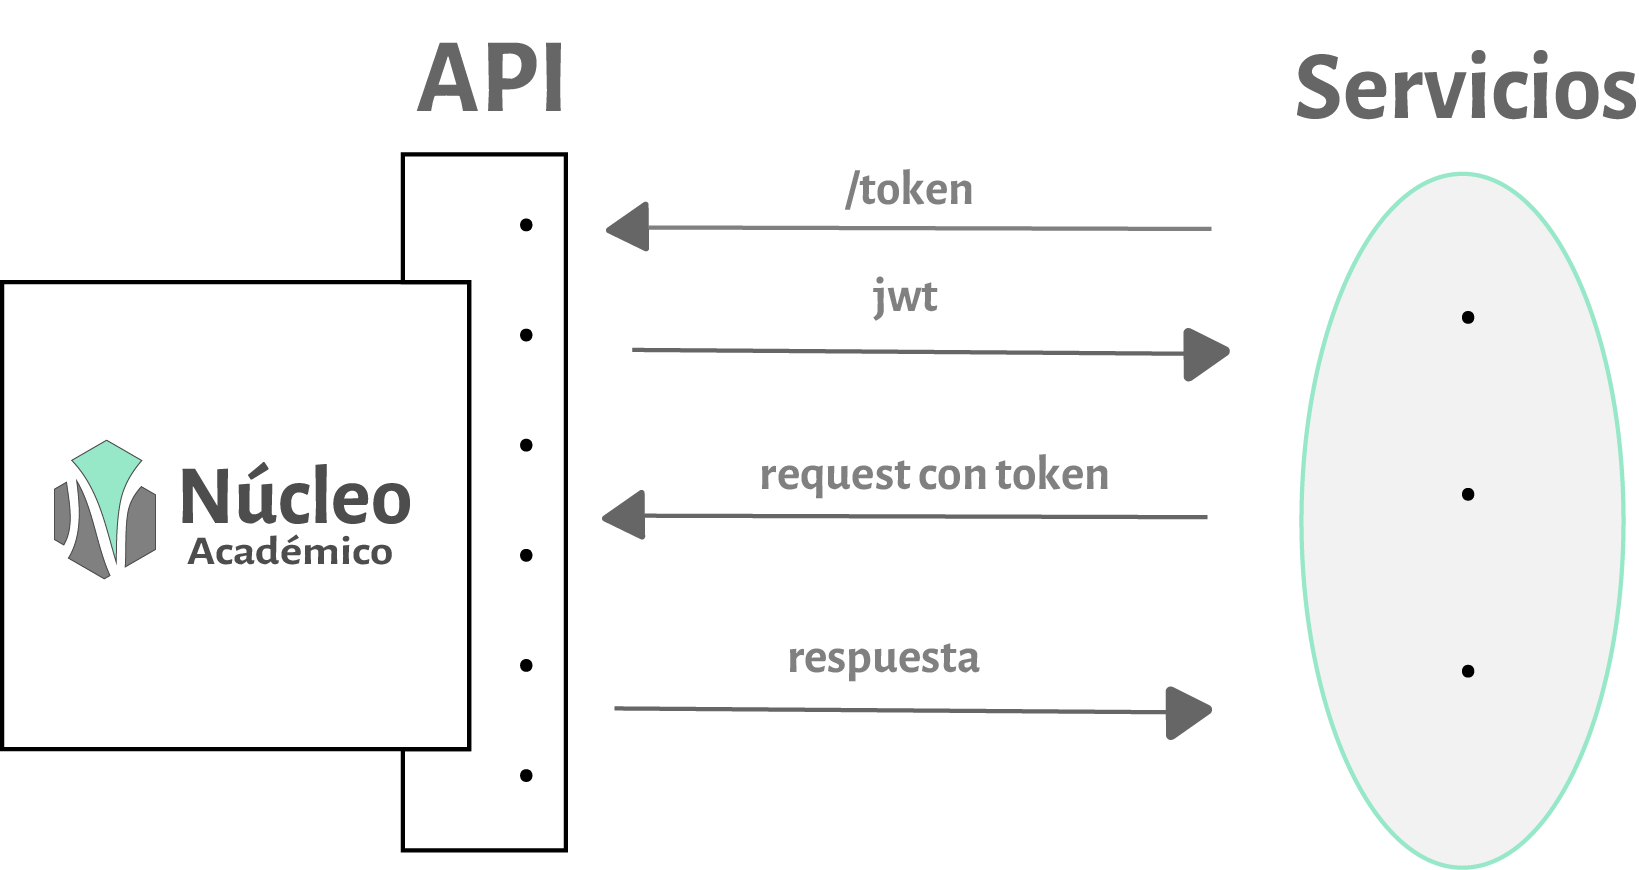
\includegraphics[scale=0.8]{images/nucleo/jwt.png}
  \captionof{figure}{Funcionamiento del pedido de token y posteriores requests}
  \label{fig:nucleo-jwt}
\end{figure}


\subsection{Deploy}

Docker, nginx, base de datos

\section[Análisis de Datos]{Análisis de Datos}

\subsection{Tecnologías}

\subsection{API REST}

\subsection{}

\section[Visualización de los datos analizados]{Visualización de los datos analizados}

\subsection{Tecnologías}

